\documentclass{article}


\usepackage{arxiv}

\usepackage[utf8]{inputenc} % allow utf-8 input
\usepackage[T1]{fontenc}    % use 8-bit T1 fonts
\usepackage[hidelinks]{hyperref}       % hyperlinks
\usepackage{url}            % simple URL typesetting
\usepackage{booktabs}       % professional-quality tables
\usepackage{amsfonts}       % blackboard math symbols
\usepackage{nicefrac}       % compact symbols for 1/2, etc.
\usepackage{microtype}      % microtypography
\usepackage{lipsum}
\usepackage{amsthm}
\usepackage{amsmath}
\usepackage{eucal}
\usepackage{mathtools}
\usepackage[table]{xcolor}
\usepackage{stmaryrd}
\usepackage{amsfonts}
\usepackage{lstlistings-golang}
\usepackage{caption}

% Code with syntax highlighting
\usepackage{fancyvrb}
\usepackage{listingsutf8}
\usepackage{textcomp}
\usepackage{placeins}


\theoremstyle{plain}% default
\newtheorem{thm}{Theorem}[section]
\newtheorem{lem}[thm]{Lemma}
\newtheorem{prop}[thm]{Proposition}
\newtheorem*{cor}{Corollary}
\theoremstyle{definition}
\newtheorem{defn}{Definition}[section]
\newtheorem{conj}{Conjecture}[section]
\newtheorem{exmp}{Example}[section]
\newtheorem{exrc}[exmp]{Exercise}
\theoremstyle{remark}
\newtheorem*{comm}{Comment}
\newtheorem*{note}{Note}
\newtheorem{case}{Case}

\def\C{\mathbb{C}}
\def\N{\mathbb{N}}
\def\Q{\mathbb{Q}}
\def\R{\mathbb{R}}
\def\Z{\mathbb{Z}}
\def\K{\mathbb{K}}

\DeclarePairedDelimiter\sqmap{\llbracket}{\rrbracket}
\DeclarePairedDelimiter\spanset{\langle}{\rangle}


\newcommand{\diag}[1]{\text{diag}\left(#1\right)}
\newcommand{\mspan}[1]{\text{span}\left(#1\right)}
\newcommand{\dom}{\text{dom}}
\newcommand{\mker}[1]{\text{ker}\left(#1\right)}
\newcommand{\mrank}[1]{\text{rank}\left(#1\right)}
\newcommand{\llwb}{\approx_{\mathcal{L}}}
\newcommand{\langlwa}[2]{\sqmap{#1}^\mathcal{L}_{#2}}

% matrix commands
\newcommand{\vvec}[2]{
	\begin{pmatrix}
		#1 \\ #2
	\end{pmatrix}
}
\newcommand{\vvvec}[3]{
	\begin{pmatrix}
		#1 \\ #2 \\ #3
	\end{pmatrix}
}
\newcommand{\vvvvec}[4]{
	\begin{pmatrix}
		#1 \\ #2 \\ #3 \\ #4
	\end{pmatrix}
}

% Code Listings
\definecolor{vgreen}{RGB}{104,180,104}
\definecolor{vblue}{RGB}{49,49,255}
\definecolor{vorange}{RGB}{255,143,102}
\lstset{
  numbers=left,
  frame=tb,
  commentstyle=\color{mygreen},
	basicstyle=\ttfamily,
	columns=fullflexible,
  keepspaces=false,
  showstringspaces=false,
  extendedchars=true,
  mathescape=true,
  breaklines, breakatwhitespace=true
}

\title{DRAFT: Go Implementation of Up-To Techniques for Weighted Language Equivalence}

%\thanks{Use footnote for providing further
%information about author (webpage, alternative
%address)---\emph{not} for acknowledging funding agencies.}

\author{
  Alessandro Cheli \\
  Undergraduate Student \\
  Department of Computer Science \\
  Università di Pisa\\
  Pisa, PI 56127 \\
  \texttt{a.cheli6@studenti.unipi.it} \\
  %% examples of more authors
  %% \And
  %% Elias D.~Striatum \\
  %% Department of Electrical Engineering\\
  %% Mount-Sheikh University\\
  %% Santa Narimana, Levand \\
  %% \texttt{stariate@ee.mount-sheikh.edu} \\
}

\definecolor{mygreen}{rgb}{0,0.6,0}



\begin{document}
\maketitle

\begin{abstract}
Weighted automata generalize non-deterministic automata by adding
a quantity expressing the weight (or probability) of the execution of each transition.
In this work we propose an implementation of two algorithms for computing language 
equivalence in finite state weighted automata (WAs). The first, a
linear partition refinement algorithm, computes the largest linear weighted bisimulation
for any given LWA (Linear Weighted Automaton) through an iterative method, 
the second algorithm checks the language equivalence 
of two vectors (states) for a given weighted automata by using an additional
data structure representing a congruence relation.
We then compare results of the two algorithms to verify their correctness
and performance on randomly generated samples. 
We finally provide a comparison and runtime statistics.
\end{abstract}


% keywords can be removed
\keywords{First keyword \and Second keyword \and More}


\section{Introduction}
\label{sec:intro}

Weighted automata (WAs) are a generalization of non-deterministic automata.
When reading a symbol, a non-deterministic automaton 
can transition in different states simultaneously. Weighted automata
introduce \textit{weights} over transitions, which can for example, 
represent the cost of a transition, 
or in probabilistic systems, the chance of such transition to happen.
WAs can be represented with a set of states, an output function and
a set of transition matrices, indexed over the symbols in the alphabet
the automaton can read. While those automata are typically defined over semirings,
for simplicity, our implementation will focus only on automata with 
transitions defined over the field of real numbers. 
The current configuration of a finite weighted automaton $W$,
defined on $n$ states, will be represented with a column vector of length
$n$, with values over the semiring or field on which transition weights of the
automaton $W$ are also defined. 

The goal of this work is to provide an high-performance implementation 
in the Go programming language of two different techniques 
to compute \textit{weighted language equivalence}.
Such equivalence relation is a bisimulation:
a relation $R$ is a bisimulation whenever two states $v_1, v_2$ in $R$ 
can simulate each other, resulting in a pair that is still in $R$.
Two state vectors $v_1, v_2$ in a weighted automaton are said to be 
weighted language equivalent, written as $v_1 \sim_l v_2$, when 
they simulate each other by accepting the same words with the same resulting output weights. 

The first technique we implement, 
defined in \cite{DBLP:journals/corr/Bonchi0K17}, is an up-to technique
for weighted language equivalence called HKC. It is defined for
weighted systems over arbitrary semirings and can be implemented with 
set theoretic constructs. The second technique is defined in \cite{BONCHI201277}:
a coalgebraic perspective is adopted to define a technique for language equivalence 
which exploits the linear representation of an automaton. 
This latter technique "\textit{minimizes}": by linearizing the state space of a
weighted automaton, 
it computes a basis for an entire linear relation (see definition \ref{def:linrel})
which coincides
with weighted language equivalence.
This technique for finite weighted automata over fields was first 
introduced by Michele Boreale in \cite{boreale2009weighted}.

Another example of the comparison between algorithms to compute 
language equivalence, precisely between HKC and an alternative
algorithm called the antichain algorithm (\cite{de2006antichains}),
was published in 2017 \cite{fu2017equivalence}.


\section{Preliminaries and Notation}
\label{sec:notation}


\begin{defn}
  A \textit{weighted automaton} over a field $\K$ and an alphabet $A$ is a triple 
  $(X,o,t)$ such that $X$ is a finite set of states, 
  $t = \left\lbrace t_a : X \to \K^X\right\rbrace_{a \in A}$
  is a set of transition functions indexed over the symbols of the alphabet $A$ and 
  $o : X  \to \K$ is the output function. 
  The transition functions will be represented as $X \times X$ matrices.
  $A^*$ is the set of all words over $A$, more precisely the free monoid
  with string concatenation as the monoid operation and the empty word $\epsilon$ 
  as the identity element. We denote with $aw$ the
  concatenation of a symbol $a$ to the word $w \in A^*$.
  A weighted language is a function $\psi: A^* \to \K$.
  A function mapping each state vector into its 
  accepted language, $\sqmap{\cdot}: \K^X \to \K^{A^*}$ is defined as follows for 
  every weighted automaton:

  \begin{equation*}
    \begin{aligned}
      \forall v \in \K^X, a \in A, w \in A^* \quad \quad
      \sqmap{v}(\epsilon) = o(v) \quad \quad
      \sqmap{v}(aw) = \sqmap{t_a(v)}(w)  
    \end{aligned}
  \end{equation*}
\end{defn}

Two vectors $v_1, v_2 \in \K^{X\times 1}$ are called weighted language equivalent, 
denoted with  $v_1 \sim_l v_2 $ if and only if 
$ \sqmap {v_1} = \sqmap{v_2}$. One can extend the notion of language 
equivalence to states rather than vectors by assigning 
to each state $x \in X$ the corresponding  unit vector 
$e_x \in \K^X$. When given an initial state $i$ for a weighted automaton, 
the language  of the automaton can be defined as $\sqmap{i}$.


\begin{defn}
  A binary relation $R \subseteq X \times Y$ between two sets $X, Y$ is a 
  subset of the 
  cartesian product of the sets. A relation is called \textit{homogeneous} 
  or an \textit
  {endorelation} if it is a binary relation over $X$ and itself: 
  $R \subseteq X \times
   X$. 
  In such case, it is simply called a binary relation over $X$.
  An \textit{equivalence relation} is a binary relation that is reflexive, 
  symmetric and
  transitive. 
  An equivalence relation which is compatible with all the operations of
the algebraic structure on which it is defined on, is called a 
\textit{congruence relation}. Compatibility with the algebraic structure operations
means that algebraic operations applied on equivalent elements will still
yield equivalent elements. 

\end{defn}



\begin{defn}
  The congruence closure $c(R)$ of a relation R is the smallest congruence relation 
  $R'$ such that $R \subseteq R'$ 
\end{defn}

\begin{defn}
  \label{def:congclos}
  \textit{Generating set for the congruence closure:} \\
  Let $\K$ be a field, $X$ a finite set and $R \subseteq \K^X \times \K^X$
  a relation. Let $(v, v') \in \K^X \times \K^X$ be a pair of vectors.
  The generating set is defined as  $U_R = \left\lbrace u - u' \mid (u, u') \in R \right\rbrace$.
  Then $(v, v') \in c(R) \iff (v - v') \in U_R$
\end{defn}



%===================================================================================

We omit the coalgebraic definition for \textit{linear weighted automata} seen in 
\cite{BONCHI201277} and give a more intuitive definition, which fits our  
implementation when $\K = \R$.
In this implementation, we focus only on weighted automata defined over 
the field of real numbers $\R$. 

\begin{defn}
  A \textit{linear weighted automaton} (in short, LWA) over the field $\K$ and 
  an alphabet $A$
  is a triple  $L = (V, o, \left\lbrace t_a \right\rbrace_{a \in A})$ 
  where $V$ is a vector space representing the state space, and $\dim{(V)} = n$;
  We have that
  $o: V \to \K$ is a linear map associating to each state its output weight,
  and $t = \left\lbrace t_a \in \K^{n \times n} \right\rbrace_{a \in A}$ is
  the set of transition functions, represented with liner maps 
  that for each input $a \in A$ associate the next state, in this case a vector
  in $V$.
  As seen in \cite{boreale2009weighted}, we have that $\dim{(L)} = \dim{(V)} = n$.
\end{defn}

Given a weighted automaton, one can build a corresponding linear weighted automaton
by considering the free vector space generated by the set of states $X$ in the WA,
and by linearizing $o$ and $t$. If $X$ is finite we can use the same matrices for 
$t$ and $o$ in both the WA and the corresponding LWA.
We are only considering a finite number of states and therefore finite dimensional
vector spaces. Let $n$ be the number of states in an WA.
We have that in the corresponding LWA, the transition functions $t_a$ are still
 represented as
$\K^{n \times n}$ matrices. $o \in \K^{1 \times n}$ is represented as a row vector.
$t_a(v)$ denotes the vector obtained by multiplying the matrix $t_a$ by the column 
vector $v  \in \K^{n \times 1}$. $o(v)$ denotes the scalar $s \in \K$ obtained by 
dot product of the row vector $o$ with $v \in \K^{n \times 1}$.

\begin{defn}
  The language recognized by a vector $v \in V$ in an LWA $(V,o,t)$ is defined
  for all words $w \in A*$ as $\langlwa{v}{V}(w) = o(v_n)$ where $v_n$ is the 
  vector reached from $v$ through the composition of the transition functions
  corresponding to each symbol in $w$.
  
  \begin{equation*}
    \begin{aligned}
      \langlwa{v}{V}(w) = \begin{cases}
        o(v) & \text{if } w = \epsilon \\ 
        \langlwa{t_a(v)}{V}(w') & \text{if } w = aw' 
      \end{cases}
    \end{aligned}
  \end{equation*}
  
\end{defn}


We define the equivalence relation  $\llwb$ for a given LWA $L = (V, o, t)$ as 

\begin{equation}
  \forall v_1, v_2 \in V, \; v_1 \llwb v_2 \iff \langlwa{v_1}{V} = \langlwa{v_2}{V}
\end{equation}

Proofs are available in section 3.3 of \cite{BONCHI201277}

Language equivalence can be now expressed in terms of linear weighted 
bisimulations (LWBs for short).
Differently from weighted bisimulations, LWBs can be seen both as relations 
and as subspaces.
The subspace representation of LWBs is used in the backwards partition 
refinement algorithm 
implemented in \cite{BONCHI201277} and in this work.

\begin{defn}
  \label{def:linrel}
  \textit{Linear Relations:}\\
  Let $U$ be a subspace of $V$. The binary relation $R_U$ over $V$ is defined by
  \begin{equation*}
    \begin{aligned}
      v_1 \; R_U \; v_2 \quad \iff \quad v_1 - v_2 \in U
    \end{aligned}
  \end{equation*}
  The relation $R$ is linear if there exists a subspace $U$ such that $R = R_U$.
  A linear relation is a total equivalence relation on $V$.
\end{defn}

\begin{defn}
  \textit{Kernel of a Relation and Linear Extension} \\
  Let $R$ be a binary relation over V. 
  The \textit{kernel} of $R$, is the set 
  $\mker{R} = \left\lbrace v_1 - v_2 \mid v_1 \; R \; v_2 \right\rbrace$.
  The \textit{linear extension} of $R$, written as $R^\ell$, is defined by 
  \begin{equation*}
    \begin{aligned}
      v_1 \; R^\ell \; v_2  \quad \iff \quad (v_1 - v_2) \in \mspan{\mker{R}}
    \end{aligned}
  \end{equation*}
\end{defn}

\begin{lem}
  Let $U$ be a subspace of $V$, then $\mker{R_U} = U$
\end{lem}

\begin{defn}
  \textit{Linear Weighted Bisimulation:} \\
  Let $(V, o, t)$ be a linear weighted automaton. A linear relation 
  $R \subseteq V \times V$ is a \textit{linear weighted bisimulation} if 
  $\forall (v_1, v_2) \in R$ it holds that: 
  \begin{center}
    \begin{enumerate}
      \item $o(v_1) = o(v_2)$
      \item $\forall a \in A, \; t_a(v_1) \; R \; t_a(v_2)$
    \end{enumerate}
  \end{center}
\end{defn}

\begin{lem}
  Let $(V, o, t)$ be a linear weighted automaton. A linear relation 
  $R$ over $V$ is a linear weighted bisimulation if and only if
\end{lem}
  \begin{center}
    \begin{enumerate}
      \item $R \subseteq \mker{o}$
      \item $R$ is $t_a$-invariant $\forall a \in A$
    \end{enumerate}
  \end{center}

Theorem 3 in section 3.3 of \cite{BONCHI201277}, states that 
$\mker{\langlwa{-}{V}}$ is the largest linear weighted bisimulation on $V$.
As a corollary, we obtain that $\llwb$ is the largest linear weighted bisimulation.

We now introduce a lemma that will be fundamental in the next sections of this work.

\begin{lem}
  \label{lem:coincide}
  $\llwb$ coincides with $\sim_l$: 

  %Let $(X, o, t)$ be a WA and $(\K^X, o^\sharp, t^\sharp)$ the corresponding linear 
  %weighted automaton. Then $\forall x \in X, \;\; \sqmap{x} = \langlwa{x}{\K^X}$
\end{lem}

\begin{figure}[htbp!]
  \centering
  

\tikzset{every picture/.style={line width=0.75pt}} %set default line width to 0.75pt        

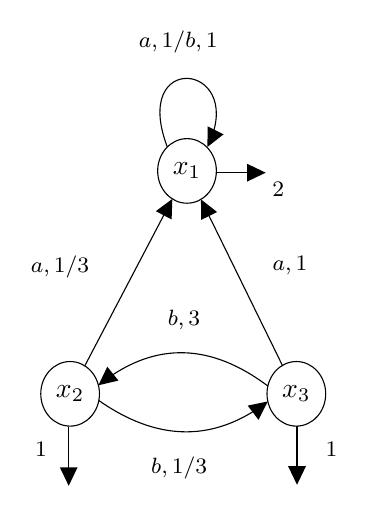
\begin{tikzpicture}[x=0.75pt,y=0.75pt,yscale=-1,xscale=1]
%uncomment if require: \path (0,514); %set diagram left start at 0, and has height of 514

%Curve Lines [id:da7520674866212254] 
\draw    (207.69,98.63) .. controls (223.51,60.79) and (169.45,55.3) .. (187,101.61) ;
\draw [shift={(206.33,101.61)}, rotate = 296.28] [fill={rgb, 255:red, 0; green, 0; blue, 0 }  ][line width=0.08]  [draw opacity=0] (8.93,-4.29) -- (0,0) -- (8.93,4.29) -- cycle    ;
%Straight Lines [id:da36516510379788225] 
\draw    (139.5,236.5) -- (139.5,261.86) ;
\draw [shift={(139.5,264.86)}, rotate = 270] [fill={rgb, 255:red, 0; green, 0; blue, 0 }  ][line width=0.08]  [draw opacity=0] (8.93,-4.29) -- (0,0) -- (8.93,4.29) -- cycle    ;
%Straight Lines [id:da06517112562563687] 
\draw    (249.5,236) -- (249.5,261.36) ;
\draw [shift={(249.5,264.36)}, rotate = 270] [fill={rgb, 255:red, 0; green, 0; blue, 0 }  ][line width=0.08]  [draw opacity=0] (8.93,-4.29) -- (0,0) -- (8.93,4.29) -- cycle    ;
%Straight Lines [id:da05488487732501923] 
\draw    (211,114) -- (231.4,114) ;
\draw [shift={(234.4,114)}, rotate = 180] [fill={rgb, 255:red, 0; green, 0; blue, 0 }  ][line width=0.08]  [draw opacity=0] (8.93,-4.29) -- (0,0) -- (8.93,4.29) -- cycle    ;

% Text Node
\draw    (196.5, 113.15) circle [x radius= 14.14, y radius= 15.56]   ;
\draw (196.5,113.15) node  [font=\normalsize]  {$x_{1}$};
% Text Node
\draw    (140.18, 220.54) circle [x radius= 14.14, y radius= 15.56]   ;
\draw (140.18,220.54) node  [font=\normalsize]  {$x_{2}$};
% Text Node
\draw    (249.18, 220.54) circle [x radius= 14.14, y radius= 15.56]   ;
\draw (249.18,220.54) node  [font=\normalsize]  {$x_{3}$};
% Text Node
\draw (178,249.9) node [anchor=north west][inner sep=0.75pt]  [font=\footnotesize]  {$b,1/3$};
% Text Node
\draw (186,178.9) node [anchor=north west][inner sep=0.75pt]  [font=\footnotesize]  {$b,3$};
% Text Node
\draw (236.5,152.9) node [anchor=north west][inner sep=0.75pt]  [font=\footnotesize]  {$a,1$};
% Text Node
\draw (172,44.4) node [anchor=north west][inner sep=0.75pt]  [font=\footnotesize]  {$a,1/b,1$};
% Text Node
\draw (120,152.9) node [anchor=north west][inner sep=0.75pt]  [font=\footnotesize]  {$a,1/3$};
% Text Node
\draw (122,242.65) node [anchor=north west][inner sep=0.75pt]  [font=\footnotesize]  {$1$};
% Text Node
\draw (262,242.65) node [anchor=north west][inner sep=0.75pt]  [font=\footnotesize]  {$1$};
% Text Node
\draw (236.4,117.4) node [anchor=north west][inner sep=0.75pt]  [font=\footnotesize]  {$2$};
% Connection
\draw    (154.02,223.76) .. controls (181.71,243.14) and (208.08,243.86) .. (233.12,225.93) ;
\draw [shift={(235.43,224.21)}, rotate = 502.59] [fill={rgb, 255:red, 0; green, 0; blue, 0 }  ][line width=0.08]  [draw opacity=0] (8.93,-4.29) -- (0,0) -- (8.93,4.29) -- cycle    ;
% Connection
\draw    (235.45,216.79) .. controls (208,196.14) and (181.57,195.41) .. (156.17,214.59) ;
\draw [shift={(153.82,216.42)}, rotate = 321.14] [fill={rgb, 255:red, 0; green, 0; blue, 0 }  ][line width=0.08]  [draw opacity=0] (8.93,-4.29) -- (0,0) -- (8.93,4.29) -- cycle    ;
% Connection
\draw    (147.25,207.06) -- (188.04,129.28) ;
\draw [shift={(189.43,126.63)}, rotate = 477.67] [fill={rgb, 255:red, 0; green, 0; blue, 0 }  ][line width=0.08]  [draw opacity=0] (8.93,-4.29) -- (0,0) -- (8.93,4.29) -- cycle    ;
% Connection
\draw    (242.46,206.85) -- (204.54,129.53) ;
\draw [shift={(203.22,126.84)}, rotate = 423.87] [fill={rgb, 255:red, 0; green, 0; blue, 0 }  ][line width=0.08]  [draw opacity=0] (8.93,-4.29) -- (0,0) -- (8.93,4.29) -- cycle    ;

\end{tikzpicture}

  \begin{equation*}
    \begin{aligned}
      o = \begin{pmatrix}
        2 & 1 & 1
      \end{pmatrix} & \quad &  
      T_a = \begin{pmatrix}
        1 & \frac{1}{3} & 1 \\ 
        0 & 0 & 0 \\
        0 & 0 & 0 \\ 
      \end{pmatrix} & \quad &
      T_b = \begin{pmatrix}
        1 & 0 & 0 \\ 
        0 & 0 & 3 \\
        0 & \frac{1}{3} & 0 \\ 
      \end{pmatrix} & \quad &
    \end{aligned}
  \end{equation*}
  \caption{Example of a Weighted Automata}
  \label{fig:autexmp}
\end{figure}

%=========================================================================


\section{Algorithms}
The first algorithm we implement to compute language equivalence, called \texttt{HKC},
is adapted from \cite{DBLP:journals/corr/Bonchi0K17}. It was first introduced by 
Bonchi and Pous in \cite{bonchi2013checking}.
The algorithm, extending the Hopcroft and Karp procedure 
\cite{hopcroft1971linear} with \textit{congruence closure}, is 
proven to be sound and complete \cite{DBLP:journals/corr/Bonchi0K17}.
Originally, the algorithm was defined for 
WAs over semirings, but we recall that in this work we are only 
considering fields, in particular 
the field of real numbers ($\K = \R$).
The problem of checking language equivalence 
has been proven undecidable for an arbitrary semiring, so termination 
may not always be guaranteed. However, it has been shown to be decidable
for a broad range of semirings, for example, all the complete and
distributive lattices.
\texttt{HKC} computes $v_1 \sim_l v_2$ for a given weighted automaton
$W = (X, t, o)$ and two vectors $v_1, v_2 \in \K^X$. 
by computing a congruence closure,
and it does so without linearizing the state space. 

We compare \texttt{HKC} with an algorithm called 
\textit{Backwards Partition Refinement}, that we will call BPR for short. 

% TODO
(TODO chiedi a filippo: nelle conclusioni di \cite{BONCHI201277} dice che è diverso 
dall'algoritmo visto nel paper di boreale \cite{boreale2009weighted}. è il caso 
anche per i field e i numeri reali???? o sono lo equivalenti?).

Adapted from \cite{BONCHI201277}, 
\texttt{BPR} is a fixed-point iterative method that, given an LWA
$L = (V, t, o)$,
computes a basis of the subspace of $V$
representing the complementary relation of $\llwb$ (we later show it to be the 
orthogonal complement in case $V$ is an inner product space). 
Another version of the algorithm is defined in the same work,
called \textit{Forward Partition Refinement}, which directly computes
a basis for $\llwb$
but is shown to be way less efficient than the backwards version.


\begin{note}
    Recall from section \ref{sec:notation} that $\llwb$ is a linear relation, 
    therefore $v_1 \llwb v_2 \iff (v_1 - v_2) \in \mker{\llwb}$
\end{note}


The \texttt{BPR} algorithm starts from a relation $R_0$, that is the complement 
of the relation identifying vectors with equal weights.
It then incrementally computes the space of all states that are reachable from 
$R_0$ in a \textit{backwards} direction. Intuitively, "going backwards" means 
working with the transpose transitions functions $t_a^t$.

In the next section we compare execution results of our implementation of the algorithms
\texttt{BPR} and \texttt{HKC} to verify the correctness of the implementation,
and to analyze when one of the two algorithms is the convenient choice.
Lemma \ref{lem:coincide}, introduced above, is key to our work. By stating that 
$\llwb$ coincides with $\sim_l$, we can confidently say that the two algorithms 
compute an answer for same the decision problem:

\begin{center}
    Are two vectors $v_1$ and $v_2$ language-equivalent for a given weighted automata? 
\end{center}

%TODO
TODO costo computazionale HKC.
\texttt{BPR} has a cost of $O(n^4)$ operations 
to initially compute the largest linear weighted bisimulation,
which can be eventually reduced to $O(n^3)$.
In our implementation, by computing a basis of the orthogonal complement of $\llwb$,
the cost of checking if two vectors are language equivalent is reduced to the
cost of matrix multiplication ($O(n^2)$). \texttt{BPR} is efficient when we
have to decide if a large number of vectors in a WA are language equivalent.

%=========================================================================

\subsection{HKC Algorithm}
We give a pseudocode definition of the \texttt{HKC} procedure:

\captionof{figure}{The \texttt{HKC}($v_1, v_2$) procedure}
\lstinputlisting[escapeinside={(*}{*)}]{hkc.txt}
\label{fig:hkc}

\subsection{Backwards Partition Refinement Algorithm for the Largest Weighted Bisimulation}
\label{sec:algo2}

We now recall the backwards algorithm for computing $\llwb$ defined in \cite{BONCHI201277}.
The algorithm is defined by the iterative method:
\begin{eqnarray}
  R_0 = \mker{o}^0, & \quad & R_{i+1} = R_i + \sum_{a \in A} t_a^t(R_i) \label{back} 
\end{eqnarray}
Where $\mker{o}^0$ is an annihilator.
The algorithm stops when $R_{j+1} = R_j$. An index $j \leq \dim(V)$ is 
guaranteed to exist, such that the algorithms terminates at step $j$.
It follows that $\llwb = R_j^0$.
Proof is available in section 4.2 of \cite{BONCHI201277}


\section{Implementation}
\label{sec:impl}

The algorithms and data structures are implemented in the Go programming 
language. Real numbers are implemented with double precision floating point numbers,  
precisely of \texttt{float64} type.

This implementation makes use of the Gonum library, 
an excellent toolkit for high-performance numerical computations.
We only import the Gonum libraries for matrices, linear algebra 
and visual plotting.
Although not GPU accelerated, Gonum matrix operations are run on 
the CPU and accelerated with BLAS and LAPACK.


\subsection{Data Structures}
In this implementation, the data structure for representing weighted automata is a \texttt{struct} containing
the following attributes:
\begin{enumerate}
    \item An integer \texttt{Dim} representing the number of states $n$. 
    (note: states are finite and indexed on natural numbers $0, \hdots, n-1$)
    \item A slice of strings representing the \textit{alphabet} $A$.
    \item A map of strings as keys (the alphabet symbols) and dense $n \times n$ \texttt{float64} matrices as values,
    representing the set of transition functions.
    \item A dense \texttt{float64} vector, representing the linearization of the output function. 
    \item A \texttt{float64} value representing the tolerance to be used in numerical computations.
    \item An optionally \texttt{nil}, dense floating point matrix providing a basis for the orthogonal 
    complement of $\llwb$
\end{enumerate}
\begin{note}
    \textit{Slices} in Go are a convenient and efficient extension of the concept of arrays: 
    they provide an abstraction for indexed, variable length sequences of typed data, and 
    provide useful helper functions for creating, appending and selecting elements. 
\end{note}
The definition can be found in file \texttt{automata/automata.go}.
We then provide methods for reading an automaton from a text stream, applying transition
and output functions to vectors, and generating random automata with real and natural valued weights.


\subsection{Implementation of HKC}
Instead of creating dedicated structs,
we exploit the \texttt{mat.Dense} data type in Gonum to efficiently represent:
\begin{itemize}
    \item Sets of vectors with $n \times k$ dense matrices ($k$ is the number of vectors in the set)
    \item Pairs of vectors with $n \times 2$ dense matrices
    \item Sets and the "\texttt{todo}" stack of pairs with $n \times 2k$ dense matrices ($k$ is the number of pairs in the set or stack)
\end{itemize}

To increase efficiency of the methods for inclusion checking and insertion in sets of vectors,
one could keep the columns ordered (by vector norm) in the corresponding matrix. 

To represent the congruence relation $R$, we introduce a \texttt{struct} containing:
\begin{itemize}
    \item A dense matrix \texttt{s} of size $n \times 2k$ containing the set of pairs in the relation
    \item A dense matrix \texttt{u} to represent the generating set $U_R$ for the congruence closure (see definition \ref{def:congclos}).
    \item Two integers representing the number of pairs in the set, and the size of vectors.
    \item A tolerance value to be used in equivalence checks. Best results were obtained with $10^{-14}$.
\end{itemize}

When adding a pair of vectors to the congruence relation, we extend the columns
of the matrix \texttt{s} with the pair $(v_1, v_2)$, if and only if $(v_1 - v_2)$ 
is not already in $U$. To check if the pair is in the congruence closure $c(R)$, 
we check if $(v_1 - v_2)$ is contained in U.

\captionof{figure}{Implementation of the \texttt{HKC}$(v_1,v_2)$ procedure}
\lstinputlisting[language=go]{../automata/hkc.go}


%TODO sistema

\subsection{Implementation of BPR}
Given a WA $L$, at the first step of \texttt{BPR}, we set $R_0 = o$, 
with $o$ being the dense vector representing the output function 
of $L$, as seen in \cite{BONCHI201277}.
For each step $i = 0, \hdots, j+1$, with $j \leq \dim(L)$, the implemented algorithm:
\begin{enumerate}
    \item For each $a \in A$ computes $t_a^T(R_i)$ through matrix multiplication
    \item Concatenates those matrices $t_a^T(R_i)$ to $R_i$ in a resulting matrix $G$ 
    \item Instead of checking linear independence of the columns through Gaussian elimination,
    it computes $R_{i+1}$ as the orthonormal basis of the column space of $G$, through singular 
    value decomposition.
\end{enumerate}

At the end of \texttt{BPR}, we store the basis for the orthogonal complement
of $\llwb$ as an attribute of the automaton. To check if two vectors $v_1 \llwb v_2$,
we check that $R_j^T(v_1 - v_2) = \vec{0}$, with a prefixed tolerance.


To compute a basis for $\llwb$, at the last step of the algorithm,
we would need to compute $R_j^0$.
If $V$ is a vector space and $W$ is a
subspace of $W$, the annihilator of $W$, respectively $W^0$ is 
a subspace of the space $V^*$ of linear functionals on $V$.
$W^0$ are the functionals that annihilate on $W$. Since 
we are working on subspaces of $\R^n$, we can directly compute 
the orthogonal complement in our implementation instead of the
annihilator.


\begin{prop}
  If $V$ is a finite dimensional vector space defined with an inner product
  $\langle \cdot , \cdot \rangle$ and $W$ is a subspace of $V$
  then the image of the annhilator $W^0$ through the linear 
  isomorphism $\varphi: V^* \to V$ induced by the inner product, 
  is the orthogonal of $W$ with respect to the said inner product.
\end{prop}

\begin{proof}
  Let $V$ be an inner product space over the field $\K$ with an inner product defined as
  $\langle \cdot , \cdot \rangle : V \times V \to \K$. 
  Every linear functional can be 
  represented with a vector. Let $\xi : V \to \K$ be a functional, 
  $\xi \in  W^0$. Because $\xi(w)=0 \quad \forall  w \in W$, 
  if $v$ represents $\xi$ we have that $(v, w)=\xi(w)=0$ for all $w \in W$. 
  We obtain that $\varphi(W^0) \subseteq W^{\perp}$.
  If $v \in W^\perp$  
  then the functional $x \mapsto (v, x)$ cancels over $W$ 
  (by the definition of orthogonality).
\end{proof}

To compute the orthogonal complement of a vector subspace $W$, we
compute $W^\perp = \mker{A^T}$, where $A$ is the matrix whose column space 
is $W$. Proof is available in \cite{ila}.


\captionof{figure}{Implementation of Backwards Partition Refinement}
\lstinputlisting[language=go]{../automata/backwards.go}

\begin{note}
    \textbf{Applications of SVD} \\
  
    Let's consider the singular value decomposition of a matrix $A \in \R^{m \times n}$:
  
    \begin{equation*}
      \begin{aligned}
        A = U \Sigma V^T & \quad & \Sigma = \diag{\sigma_1, \sigma_2, \hdots, \sigma_r  } 
         & \quad &  U \in \R^{m \times m} & \quad & V \in \R^{n \times n}
      \end{aligned}
    \end{equation*}
  
    Where $V$ and $U$ are orthogonal and the singular values are ordered: $\sigma_1 \geq \sigma_2 \geq \hdots \geq \sigma_r \geq 0$.
    It follows that $\mrank{A}$ is equal to the number of nonzero singular values, and
    as explained in \cite{svd}:
    
    \begin{enumerate}
      \item  $\mrank{A} = \mrank{\Sigma} = r$
      \item The column space of $A$ is spanned by the first $r$ columns of $U$.
      \item The null space of $A$ is spanned by the last $n − r$ columns of $V$.
      \item The row space of $A$ is spanned by the first $r$ columns of $V$.
      \item The null space of $A^T$ is spanned by the last $m − r$ columns of $U$.
    \end{enumerate}
    
    Of our interest, are only the computation of the null space and column space.
    The implementation 
    can be found in files \texttt{lin/colspace.go} and \texttt{lin/nullspace.go}.
  \end{note}



\section{Runtime Results}

%TODO da fare e sistemare.

%\subsection{Tolerance and F1 Score}
We the studied of the influence 
of the tolerance value over the correctness of the algorithms results.
Tests took place on randomly generated automata. A basis of  $\llwb$ was 
computed for each automaton with BPR. An arbitrary number of vector pairs were generated 
as uniformly distributed random linear combinations of the vectors in the spanning set of $\llwb$. 
The same quantity of vector pairs was generated randomly with an uniform distribution.
BPREquivalence and HKC procedures were then executed with those pairs in input.

By defining pairs of vectors as 

\begin{itemize}
    \item \textit{true positives} (TP) if reported as language equivalent by both 
    procedures
    \item \textit{true negatives} (TN) if reported as not language equivalent by both 
    procedures
    \item \textit{false positives} (FP) if reported as language equivalent by HKC but not by BPR
    \item \textit{false negatives} (FN) if reported as  language equivalent by BPR but not by HKC
\end{itemize}


We then borrow four concepts from binary classification: \textit{accuracy, precision, recall} 
and \textit{F1 score}: 

\begin{equation*}
    \begin{aligned}
        \text{Accuracy} = \dfrac{TP + TN}{TP + TN + FP + FN} & \quad & 
        \text{Recall} = \dfrac{TP}{TP + FN} \\ && \\
        \text{Precision} = \dfrac{TP}{TP + FP} & \quad &
        \text{F1} = 2 \cdot \dfrac{\text{Precision} \cdot \text{Recall}}{\text{Precision} + \text{Recall}}  \\ && \\
    \end{aligned}
\end{equation*}

We have then computed 
the F1 score in relation to varying tolerance values.
The plot is shown in Figures \ref{fig:f1} and \ref{fig:f1-2}.  
The program was executed on an x86\_64 AMD Ryzen 5 2600X Six Core CPU, running at 3.6GHz with 32GB RAM, 
running Void Linux. Executed sequentially, F1 score tests took an average 2m26.19s,
Parallelized by using a worker pool, the tests lasted the times reported in 
Figure \ref{fig:f1} and \ref{fig:f1-2}.
For example, in the first plot of Figure \ref{fig:f1-2}, the test took 82 seconds.
Since we computed BPR for 3000 random automata, over 17 tolerance values, for 3 line plots,
with a chance of finding a non-empty basis for $\llwb$ of approximately $1/3$,
the BPR algorithm was executed an approximate average of
$\frac{3000 \cdot 3 \cdot 17}{82} \approx 1865$ times per second. 
The HKC algorithm, was executed 2000 times on each automaton with a non-empty 
basis of $\llwb$, therefore, it was executed an approximate average of 
$\frac{3000 \cdot 17 \cdot 2000 \cdot 3}{3 \cdot 82} \approx 1243902$ times per second.

% //TODO: condizionamento BPR
%TODO: BPR conditioning

\begin{figure}[htbp!]
    \centering
    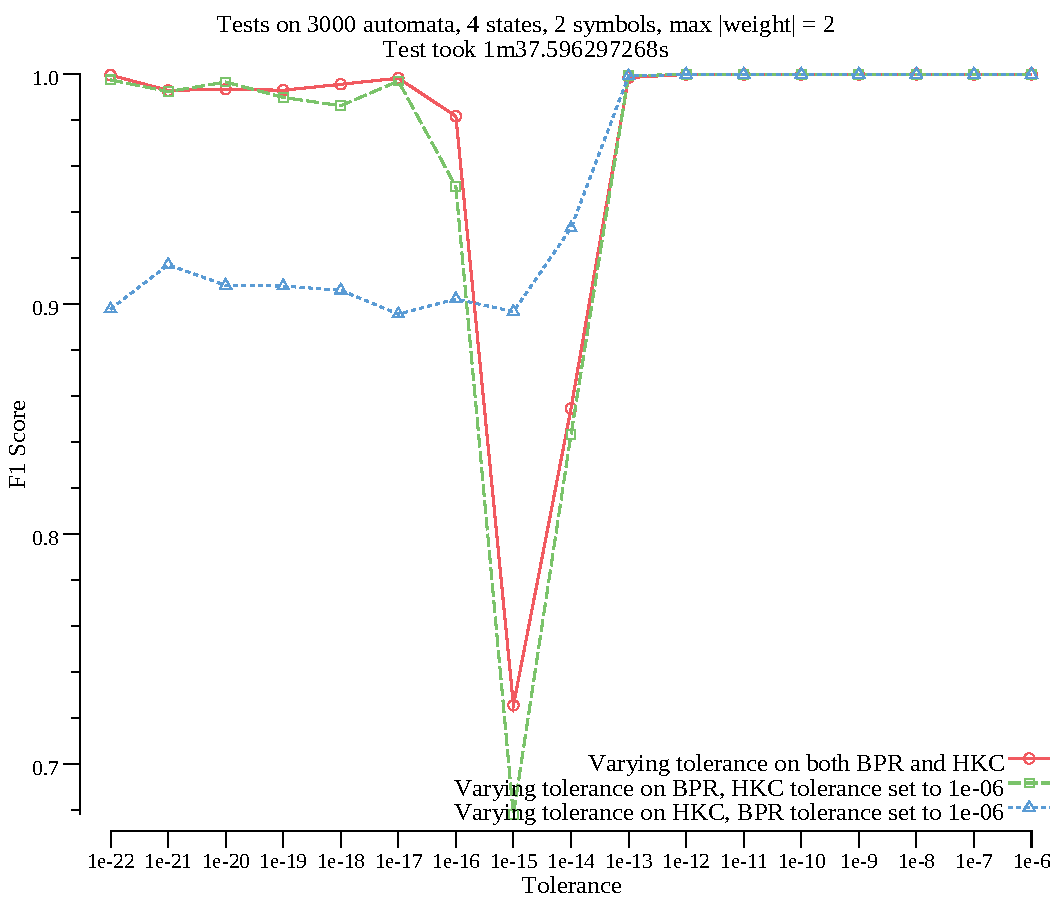
\includegraphics[width=.75\textwidth]{./plots/f1-tol-1e-06.pdf}
    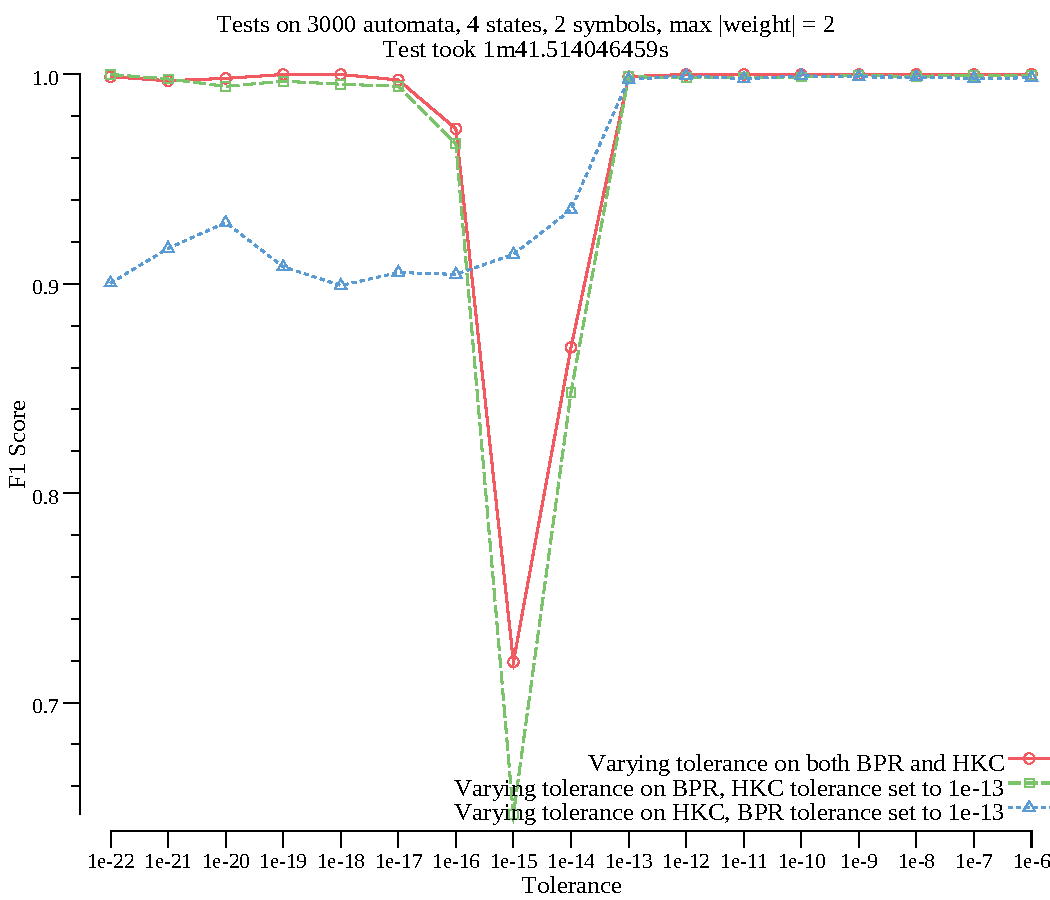
\includegraphics[width=.75\textwidth]{./plots/f1-tol-1e-13.pdf}
    \caption{F1 score over tolerance tests, 2000 vector pairs tested per automaton.}
    \label{fig:f1}
\end{figure}

\begin{figure}[htbp!]
    \centering
    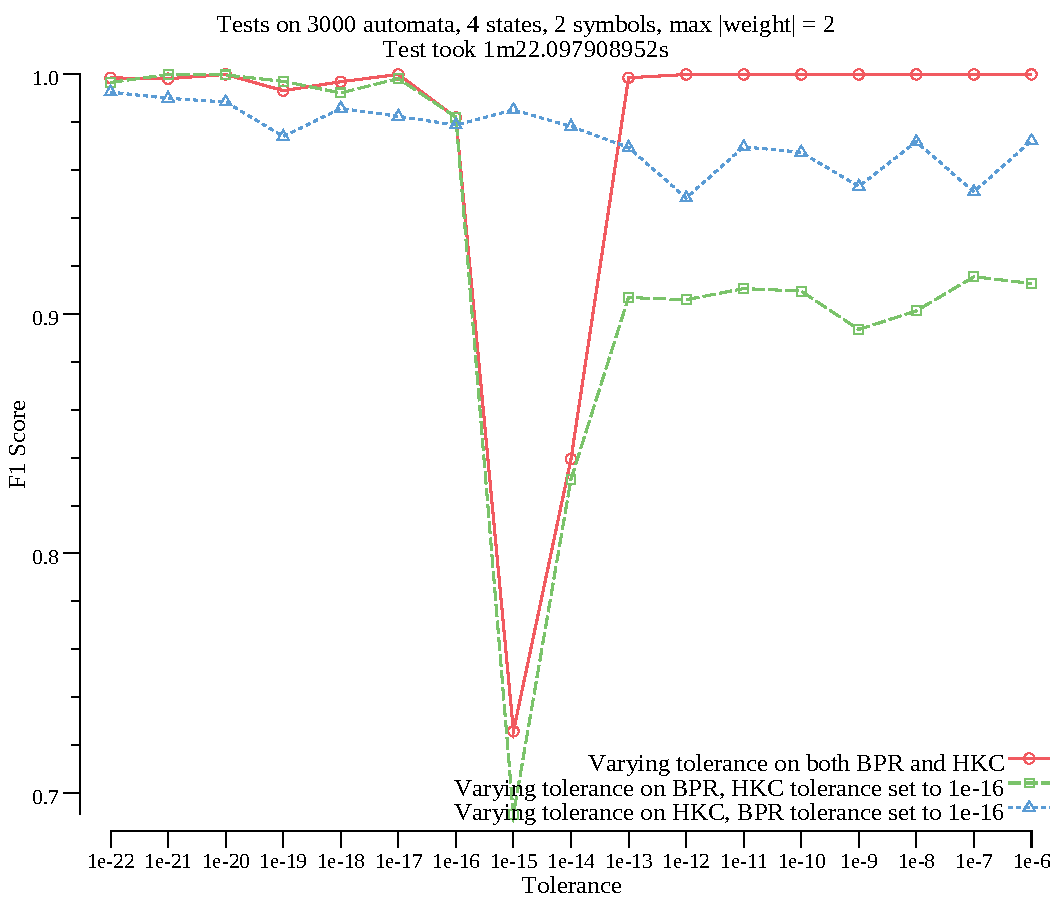
\includegraphics[width=.75\textwidth]{./plots/f1-tol-1e-16.pdf}
    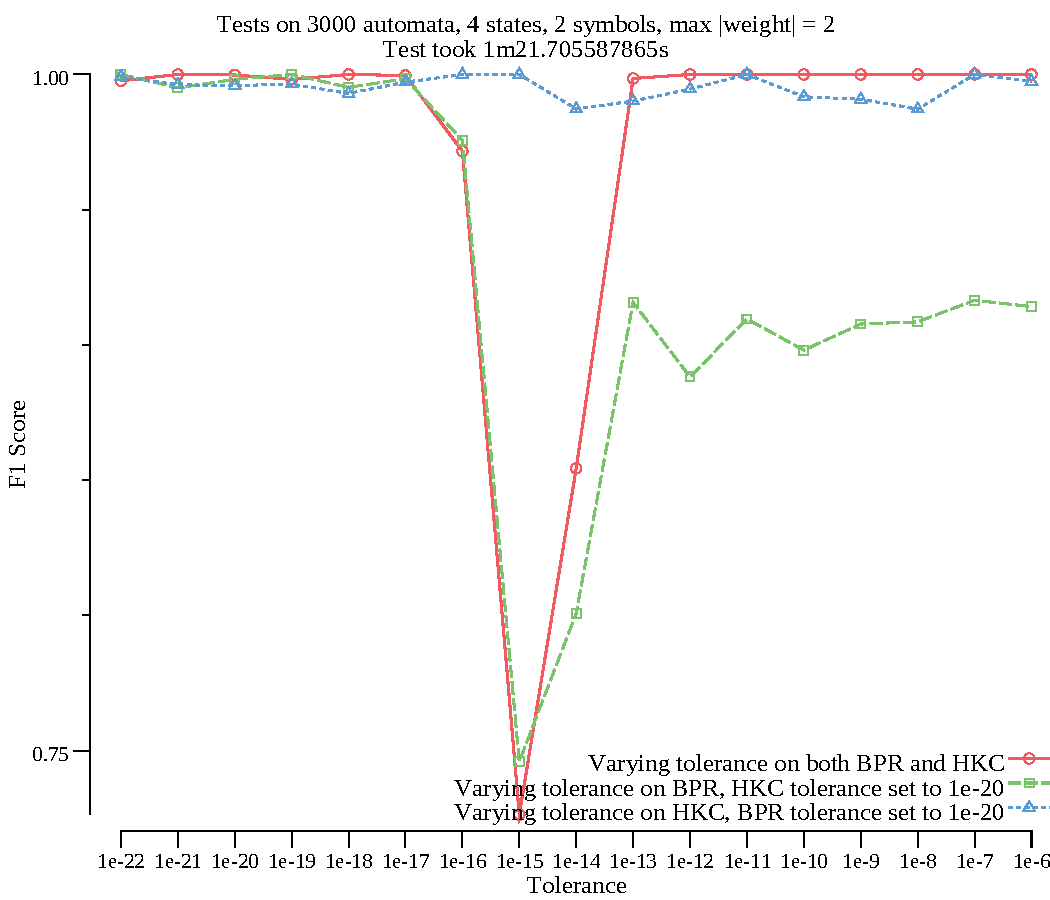
\includegraphics[width=.75\textwidth]{./plots/f1-tol-1e-20.pdf}
    \caption{F1 score over tolerance tests, 2000 vector pairs tested per automaton.}
    \label{fig:f1-2}
\end{figure}


%TODO empty LLWB chance, memory and time plots, varying automata size parameters

\section{Conclusion and Future Work}


During the testing phase, we have found that on randomly generated automata 
over the $\R$ field, the probability of BPR returning an empty basis of $\llwb$
increases together with the number of states in the automaton, and the number of
 symbols in the alphabet.
In a given linear weighted automaton $L = (V, o,t )$
over the $\R$ field and an alphabet $A$, the chance of BPR returning an empty basis also
increases together with the maximum weight in modulo of the transition matrices,
$\forall a \in A, \; \max |(t_a)_{ij}|$, for $i,j=1\hdots,n$, with 
$n = \dim(V)$. Authors of \cite{BONCHI201277} have confirmed
that it is normal for this to happen and that this fact is not due
to an implementation error.

Since the tests in this work rely heavily on a non-empty basis of $\llwb$ to generate
language equivalent vectors, the automata with an empty $\mker{\llwb}$ had to be ignored during the 
tests. This introduced substantial overhead as the chance of BPR returning an empty basis 
grew closer to 1, together with the various parameter of the automata: 
most of the computing time was spent on generating and running BPR on automata which did
not contain any language equivalent vectors, making tests on large automata not possible.

To provide better runtime results for the language equivalence problem, 
a topic worth further attention is the development of a semi-randomized method to 
generate structured large sized automata that have a low chance of BPR
returning an empty basis of $\llwb$.

Another topic worth further investigation is the cause of the 
sudden drop at 1e-15 in the F1 score plots.


An idea for the future of this implementation, is the addition
of a \texttt{Semiring} interface type that would permit much more insightful analysis
on weighted automata, not only on the field of real numbers.  

To further verify of the algorithms implemented in this work, 
and any additional algorithm that may be implemented, 
one could compare the results of this package with the results 
of the PAWS tool for the analysis of weighted systems \cite{konig2017paws}, developed 
at the University of Duisburg-Essen.



%=============================================================


%\begin{figure}
%  \centering
%  \fbox{\rule[-.5cm]{4cm}{4cm} \rule[-.5cm]{4cm}{0cm}}
%  \caption{Sample figure caption.}
%  \label{fig:fig1}
%\end{figure}


%\begin{table}
% \caption{Sample table title}
%  \centering
%  \begin{tabular}{lll}
%    \toprule
%    \multicolumn{2}{c}{Part}                   \\
%    \cmidrule(r){1-2}
%    Name     & Description     & Size ($\mu$m) \\
%    \midrule
%    Dendrite & Input terminal  & $\sim$100     \\
%    Axon     & Output terminal & $\sim$10      \\
%    Soma     & Cell body       & up to $10^6$  \\
%    \bottomrule
%  \end{tabular}
%  \label{tab:table}
%\end{table}





\bibliographystyle{unsrt}
\bibliography{references} 

\appendix

%\section{Complete Code}

\subsection{Linear Algebra Utilities}

\captionof{figure}{\texttt{lin/util.go}}
\lstinputlisting[language=go]{../lin/util.go}

\captionof{figure}{\texttt{lin/subspace.go}}
\lstinputlisting[language=go]{../lin/subspace.go}

\captionof{figure}{\texttt{lin/independent.go}}
\lstinputlisting[language=go]{../lin/independent.go}

\captionof{figure}{\texttt{lin/nullspace.go}}
\lstinputlisting[language=go]{../lin/nullspace.go}

\captionof{figure}{\texttt{lin/colspace.go}}
\lstinputlisting[language=go]{../lin/colspace.go}


\subsection{Automata Data Structures and Methods}

\captionof{figure}{automata/automata.go}
\lstinputlisting[language=go]{../automata/automata.go}

\captionof{figure}{automata/io.go}
\lstinputlisting[language=go]{../automata/io.go}

\captionof{figure}{automata/random.go}
\lstinputlisting[language=go]{../automata/random.go}

\subsection{Pair, Relation and To-Do list Structures and Methods}


\captionof{figure}{automata/pair.go}
\lstinputlisting[language=go]{../automata/pair.go}

\captionof{figure}{automata/pairstack.go}
\lstinputlisting[language=go]{../automata/pairstack.go}

\captionof{figure}{automata/relation.go}
\lstinputlisting[language=go]{../automata/relation.go}


\subsection{Algorithms}

\captionof{figure}{automata/hkc.go}
\lstinputlisting[language=go]{../automata/hkc.go}

\captionof{figure}{automata/backwards.go}
\lstinputlisting[language=go]{../automata/backwards.go}


\subsection{Main Package}

\captionof{figure}{\texttt{randtest/randtest.go}}
\lstinputlisting[language=go]{../randtest/randtest.go}


\captionof{figure}{\texttt{main.go}}
\lstinputlisting[language=go]{../main.go}


\section{Test Files}

\end{document}
 